\subsection{Version control system}

\subsubsection{Apache Subversion}
Apache Subversion (often abbreviated SVN, after the command name svn) is a software versioning and a revision control system distributed under a free license. Developers use Subversion to maintain current and historical versions of files such as source code, web pages, and documentation.\cite{wiki:svn}

Subversion repositories can be hosted by Google Code or at IDI through Gurutjenesten. SVN has good tools for eclipse, making it easy for developers to use its powerful features.

\subsubsection{Git}
Git is a distributed revision control system with an emphasis on speed. Git was initially designed and developed by Linus Torvalds for Linux kernel development. Every Git working directory is a full-fledged repository with complete history and full revision tracking capabilities, not dependent on network access or a central server. Git is free software distributed under the terms of the GNU General Public License version 2.\cite{wiki:git}

For developers, git is better at merging branches, and merging in general. Being a command-line focused tool makes it a bit harder to use for inexperienced developers, or developers unfamiliar with the command-line. Some GUI clients do exists, but they do not always implement the entire rich features of git. 

The biggest asset of Git is GitHub. GitHub is a web-based hosting service for software development projects that use the Git revision control system. The site provides social networking functionality such as feeds, followers and the network graph to display how developers work on their versions of a repository.\cite{wiki:github} In addition, GitHub now features one of the best issue trackers available, making it a powerful tool for any developer team.

\begin{figure}[htb]
	\centering
	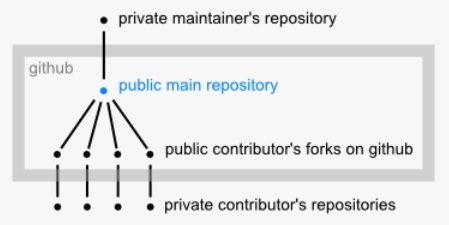
\includegraphics[width=0.6\textwidth]{prestudy/github.jpg}
	\caption{Distributed setup of git repositories\cite{git:repositories}}
	\label{fig:github}
\end{figure}

\subsubsection{Conclusion}
Because the project requires issue trackers and a rich commit history, the team has decided that using git is the right approach. The group has previous experience in using git, and we could get it up and running fairly quickly after project launch. The project is also Open Source, so having it as such on GitHub is not a problem.
